
\documentclass[conference]{IEEEtran}

\usepackage{float} 
\usepackage{url}  
\usepackage{multirow}
\usepackage{caption}
\usepackage{subcaption}
\usepackage{booktabs}
\usepackage{cite}
\pagestyle{plain}
\usepackage{amsmath}
\usepackage{float}
\usepackage{tikz}
\usetikzlibrary{shapes.geometric, arrows, positioning}
\usepackage{placeins}
\usepackage{comment}
\usepackage{tabularx}
\ifCLASSINFOpdf
  \usepackage[pdftex]{graphicx}
\fi

\hyphenation{op-tical net-works semi-conduc-tor}

\begin{document}


\title{Exploring financial sentiment analysis with the Financial Phrasebank dataset}

\author{\IEEEauthorblockN{\\ Hugo Veríssimo}
\IEEEauthorblockA{Complements of Machine Learning 24/25\\
University of Aveiro\\
Aveiro, Portugal\\
hugoverissimo@ua.pt}
\and
\IEEEauthorblockN{\\ João Cardoso}
\IEEEauthorblockA{Complements of Machine Learning 24/25\\
University of Aveiro\\
Aveiro, Portugal\\
joaopcardoso@ua.pt}}

\maketitle
\thispagestyle{plain}

\begin{abstract}
abstratotoototot
\end{abstract}

\begin{quote}
\small
\noindent
\textbf{Keywords:} key, word, number, 1
\end{quote}

\IEEEpeerreviewmaketitle


\section{Introduction}

With the ever increasing volume of information created and distributed by the minute, it is more important than ever to have access to fast and reliable analysis of any information we may come across. Especially with the democratized access to financial instruments and capital markets, where individuals have the possibility to invest in virtually any company on the stock exchange, it is important to have ways to leverage against giant institutions with hundreds of financial analysts at their disposal. 

\begin{figure}[H]
    \centering
    
\includegraphics[width=0.5\linewidth]{bugs.png}
    \caption{Power to the people, colorized (circa 1917).}
    \label{fig:enter-label}
\end{figure}

Historically, financial analysis relied heavily on fundamental analysis (examining earnings, balance sheets, annual financial reports), which required extensive knowledge in the field (also the strategy that made Warren Buffett one of the richest men in the world), along with technical analysis (studying price and volume trends). Around 2010, after the 2008 global financial crisis, there was a surge in news analysis to evaluate the tone and derive investment strategies from it. Due to the lack of domain specific lexicon these analysis were falible, until the work by Loughran and McDonald was published, a financial lexicon based on 10-K forms (i.e., annual financial reports) and dictionaries. This allowed to use more sofisticated analysis rather than using the presence of negative words as a signal to sell.

Upon the launch of Twitter, information streams increased dramatically, making more and more data available for analysis. But, machine learning was not heavily used, as most data was not annotated, or there was very little data with high-quality annotations. In 2014, P. Malo \textit{et al.} published a fundamental dataset for financial sentimental analysis, that is still used, the Financial Phrasebank. It is unique, for the inclusion of important aspects as directional expressions (e.g., profits decreased), entity polarity shifts (e.g. profits may be negative if decreased), and phrase level context.

With this, machine learning models started finding their place in research, as the field of natural language processing (NLP) grew and niche fields such as financial investments found useful data. In this work we explore the Financial Phrasebank dataset, by implementing different machine learning and deep learning models to evaluate the sentiment of sentences related to financial news.

\section{State of The Art}

The field of NLP has grown drastically in the past decade, progressing from recurrent neural networks (RNN) and related models such as Long-Short Term Memory (LSTM), to the transformers-type models, large language models (LLM) and text generative models as ChatGPT. With the Financial Phrasebank the field expanded into financial analysis, with several works of relevance being published in recent years.

In the work of Araci (2019), the author developed a BERT-based model trained specifically on texts with financial data. BERT, Bidireccional Encoder Representations from Transformers, is a large language model developed by Google (2018), benefitting largely from the fact that it can "hold" in memory large chunks and in both directions, simultaneously. The fact that it is built on the Transformer encoder architecture, it can weigh the importance of different words in a sentence by using a self-attention. The model is pre-trained  on large unlabelled corpora (e.g., Wikipedia, BookCorpus), and can be fine-tuned for specific purposes. In this work, the end model was trained on  domain specific corpus such as TRC2-financial data and financial specific texts (over ~440 000 sentences), and then fine tuned with the Financial Phrasebank. The model achieved an accuracy of 97 \% on the Financial Phrasebank dataset with 100 \% agreement, but 86 \% and 85 \% respectively on the dataset with all levels of agreement (the agreement will be further detailed in the Methodology section). Later on the model was further improved by Sun \textit{et al.} (2025), EnhancedFinSentiBERT, by including dictionary embeddings, expanded corpus that deversified the pre-training stage drastically, and a novel neutral sentiment module, that further enhanced the distinction between neutral and weak sentiments, resulting in improved accuracy (89 \%) and F1-score (88 \%). The pre-training stage benefited from the large diversity of the corpus, going from a few million tokens to 2.4 B tokens with the latest version.

In a similar direction, but at the fine tuning level, Atsiwo (2024) improved the data used in fine tuning, considering that most datasets have relatively short sentences ($<$ 100 tokens), failing to leverage the full context window  of LLMs like BERT (512 tokens). This was achieved by augmenting  the training data with synthetic sentences generated by GPT-4, with accuracy of 89 \% and F1-score of 88 \% for 50 \% agreement dataset.


\section{Methodology}

\subsection{Dataset}

https://huggingface.co/datasets/takala/financial\_phrasebank
\cite{dataset, malo2013gooddebtbaddebt}

The Financial PhraseBank is a widely used benchmark dataset for financial sentiment analysis. It consists of roughly 4,840 English sentences (mostly news headlines or short statements) about companies, drawn from financial news articles and press releases. Each sentence is labeled with one of three sentiment classes – positive, negative, or neutral – representing the sentence’s sentiment from the perspective of an investor.

\begin{table}[H]
\centering
\caption{data distribution}
\label{agreement_datasets}
\begin{tabular}{lcccc}
\toprule
\textbf{Sentiment} & \multicolumn{4}{c}{\textbf{Agreement}} \\
\cmidrule(lr){2-5}
 & \textbf{50\%} & \textbf{66\%} & \textbf{75\%} & \textbf{All} \\
\midrule
Negative & 604 & 514 & 420 & 303 \\
Neutral & 2879 & 2535 & 2146 & 1391 \\
Positive & 1363 & 1168 & 887 & 570 \\
\midrule
\textbf{Total} & 4846 & 4217 & 3453 & 2264 \\
\bottomrule
\end{tabular}
\end{table}

o dataset foi anotado (labels) por 16 anotadores com background em economia/finanças, sendo que cada anotou um subset de frases. cada instância foi anotada por 5-8 anotadores independentes, levando então à criação de 5 sub datasets tendo em conta o nível de concordaância entre as anotações: 50\% de agreement, 66\%, 75\%, e concordância total. a distribuição das classes juntamente com a quantidade total de instancias é apresentada na tabela \ref{agreement_datasets}. importa também referir que a cada determinada concordância é um mínimo, ou seja, por exemplo o dataset de 50\% de Agreement contem os datasets de 66\%, 75\% e total concordância.

estes subsets permitem aos investigadores ter um equilíbrio entre quantidade de dados e qualide dos dados, representando um trade-off muito comum no espaço da aprendizagem automática (ig)

% exemplos de frases

%Sentence: According to Gran , the company has no plans to move all production to Russia , although that is where the company is growing ., Label: neutral

%Sentence: For the last quarter of 2010 , Componenta 's net sales doubled to EUR131m from EUR76m for the same period a year earlier , while it moved to a zero pre-tax profit from a pre-tax loss of EUR7m ., Label: positive

%Sentence: In the third quarter of 2010 , net sales increased by 5.2 \% to EUR 205.5 mn , and operating profit by 34.9 \% to EUR 23.5 mn ., Label: positive

%Sentence: Operating profit totalled EUR 21.1 mn , up from EUR 18.6 mn in 2007 , representing 9.7 \% of net sales ., Label: positive

\subsection{Exploratory Data Analysis}

tendo em conta os vários subsets dispobíveis do Financial Phrasebank, o escolhido para análise mais detalhada ao longo deste projeto foi o dataset 75Agreement, representado possivelmente o melhor equilibrio entre qualidade e quantidade, tendo em conta a qnt de instancia por classe face às restantes concordâncias.

\begin{figure}[H]
    \centering
    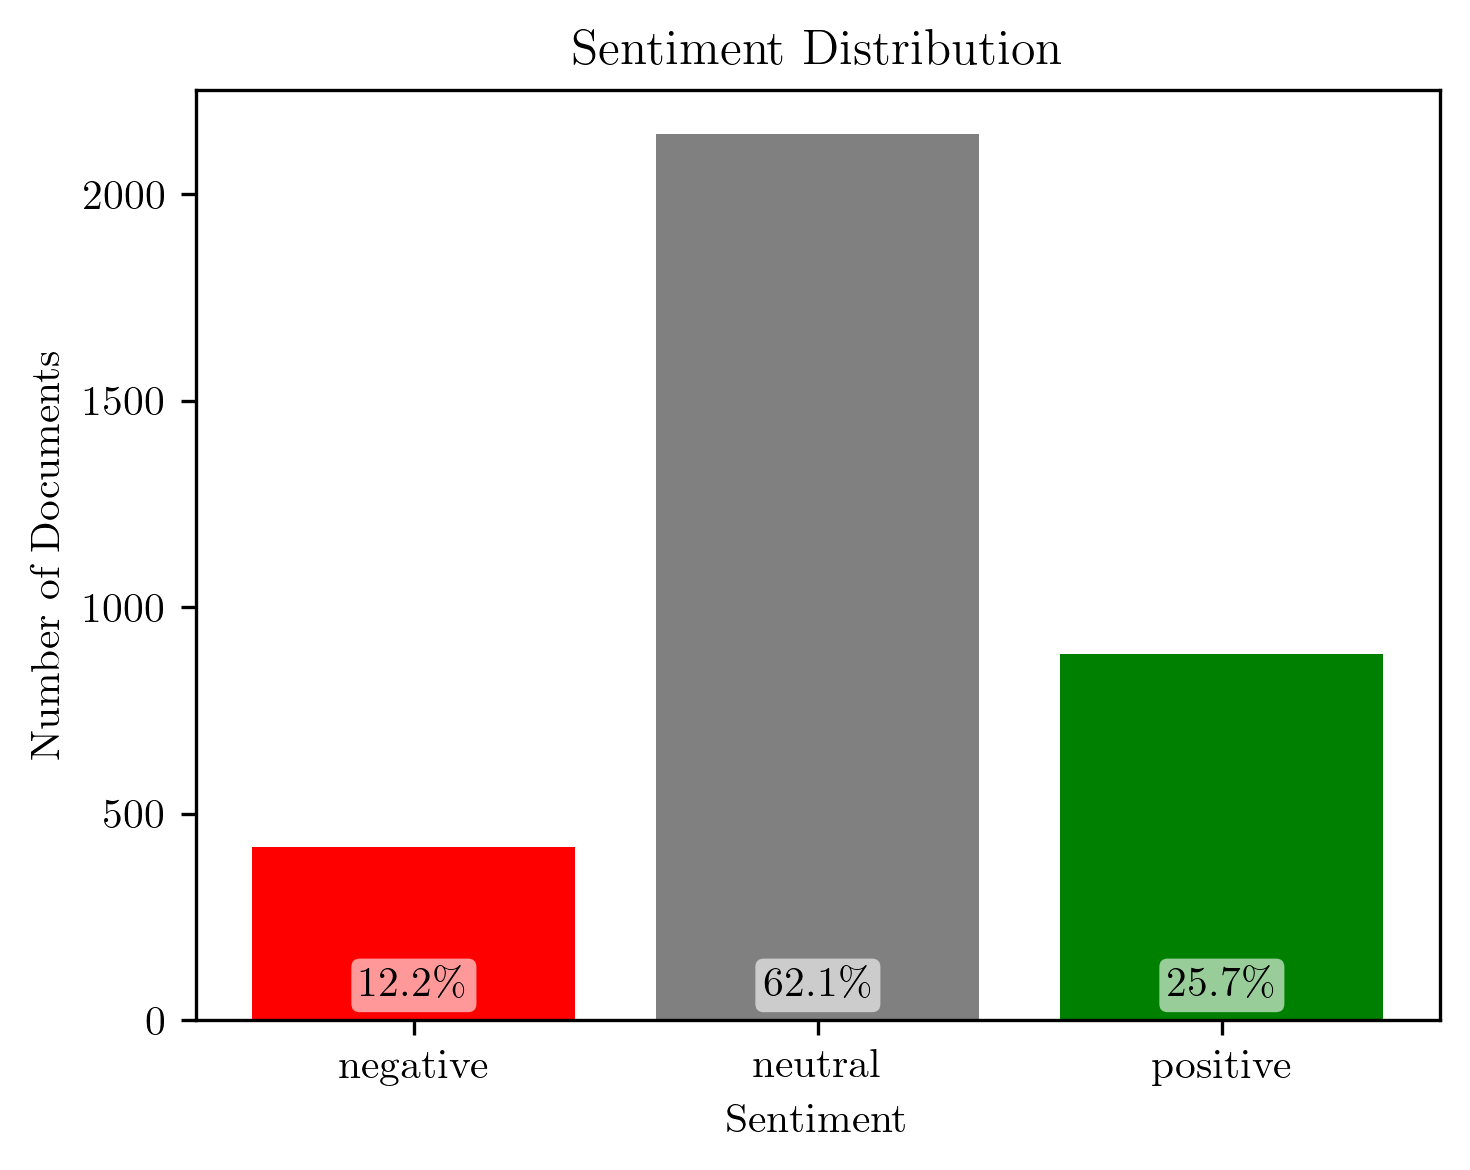
\includegraphics[width=1\linewidth]{assets/sentiment_distribution.png}
    \caption{classes distribution}
    \label{fig:sentiment_distribution}
\end{figure}

\begin{figure}[H]
    \centering
    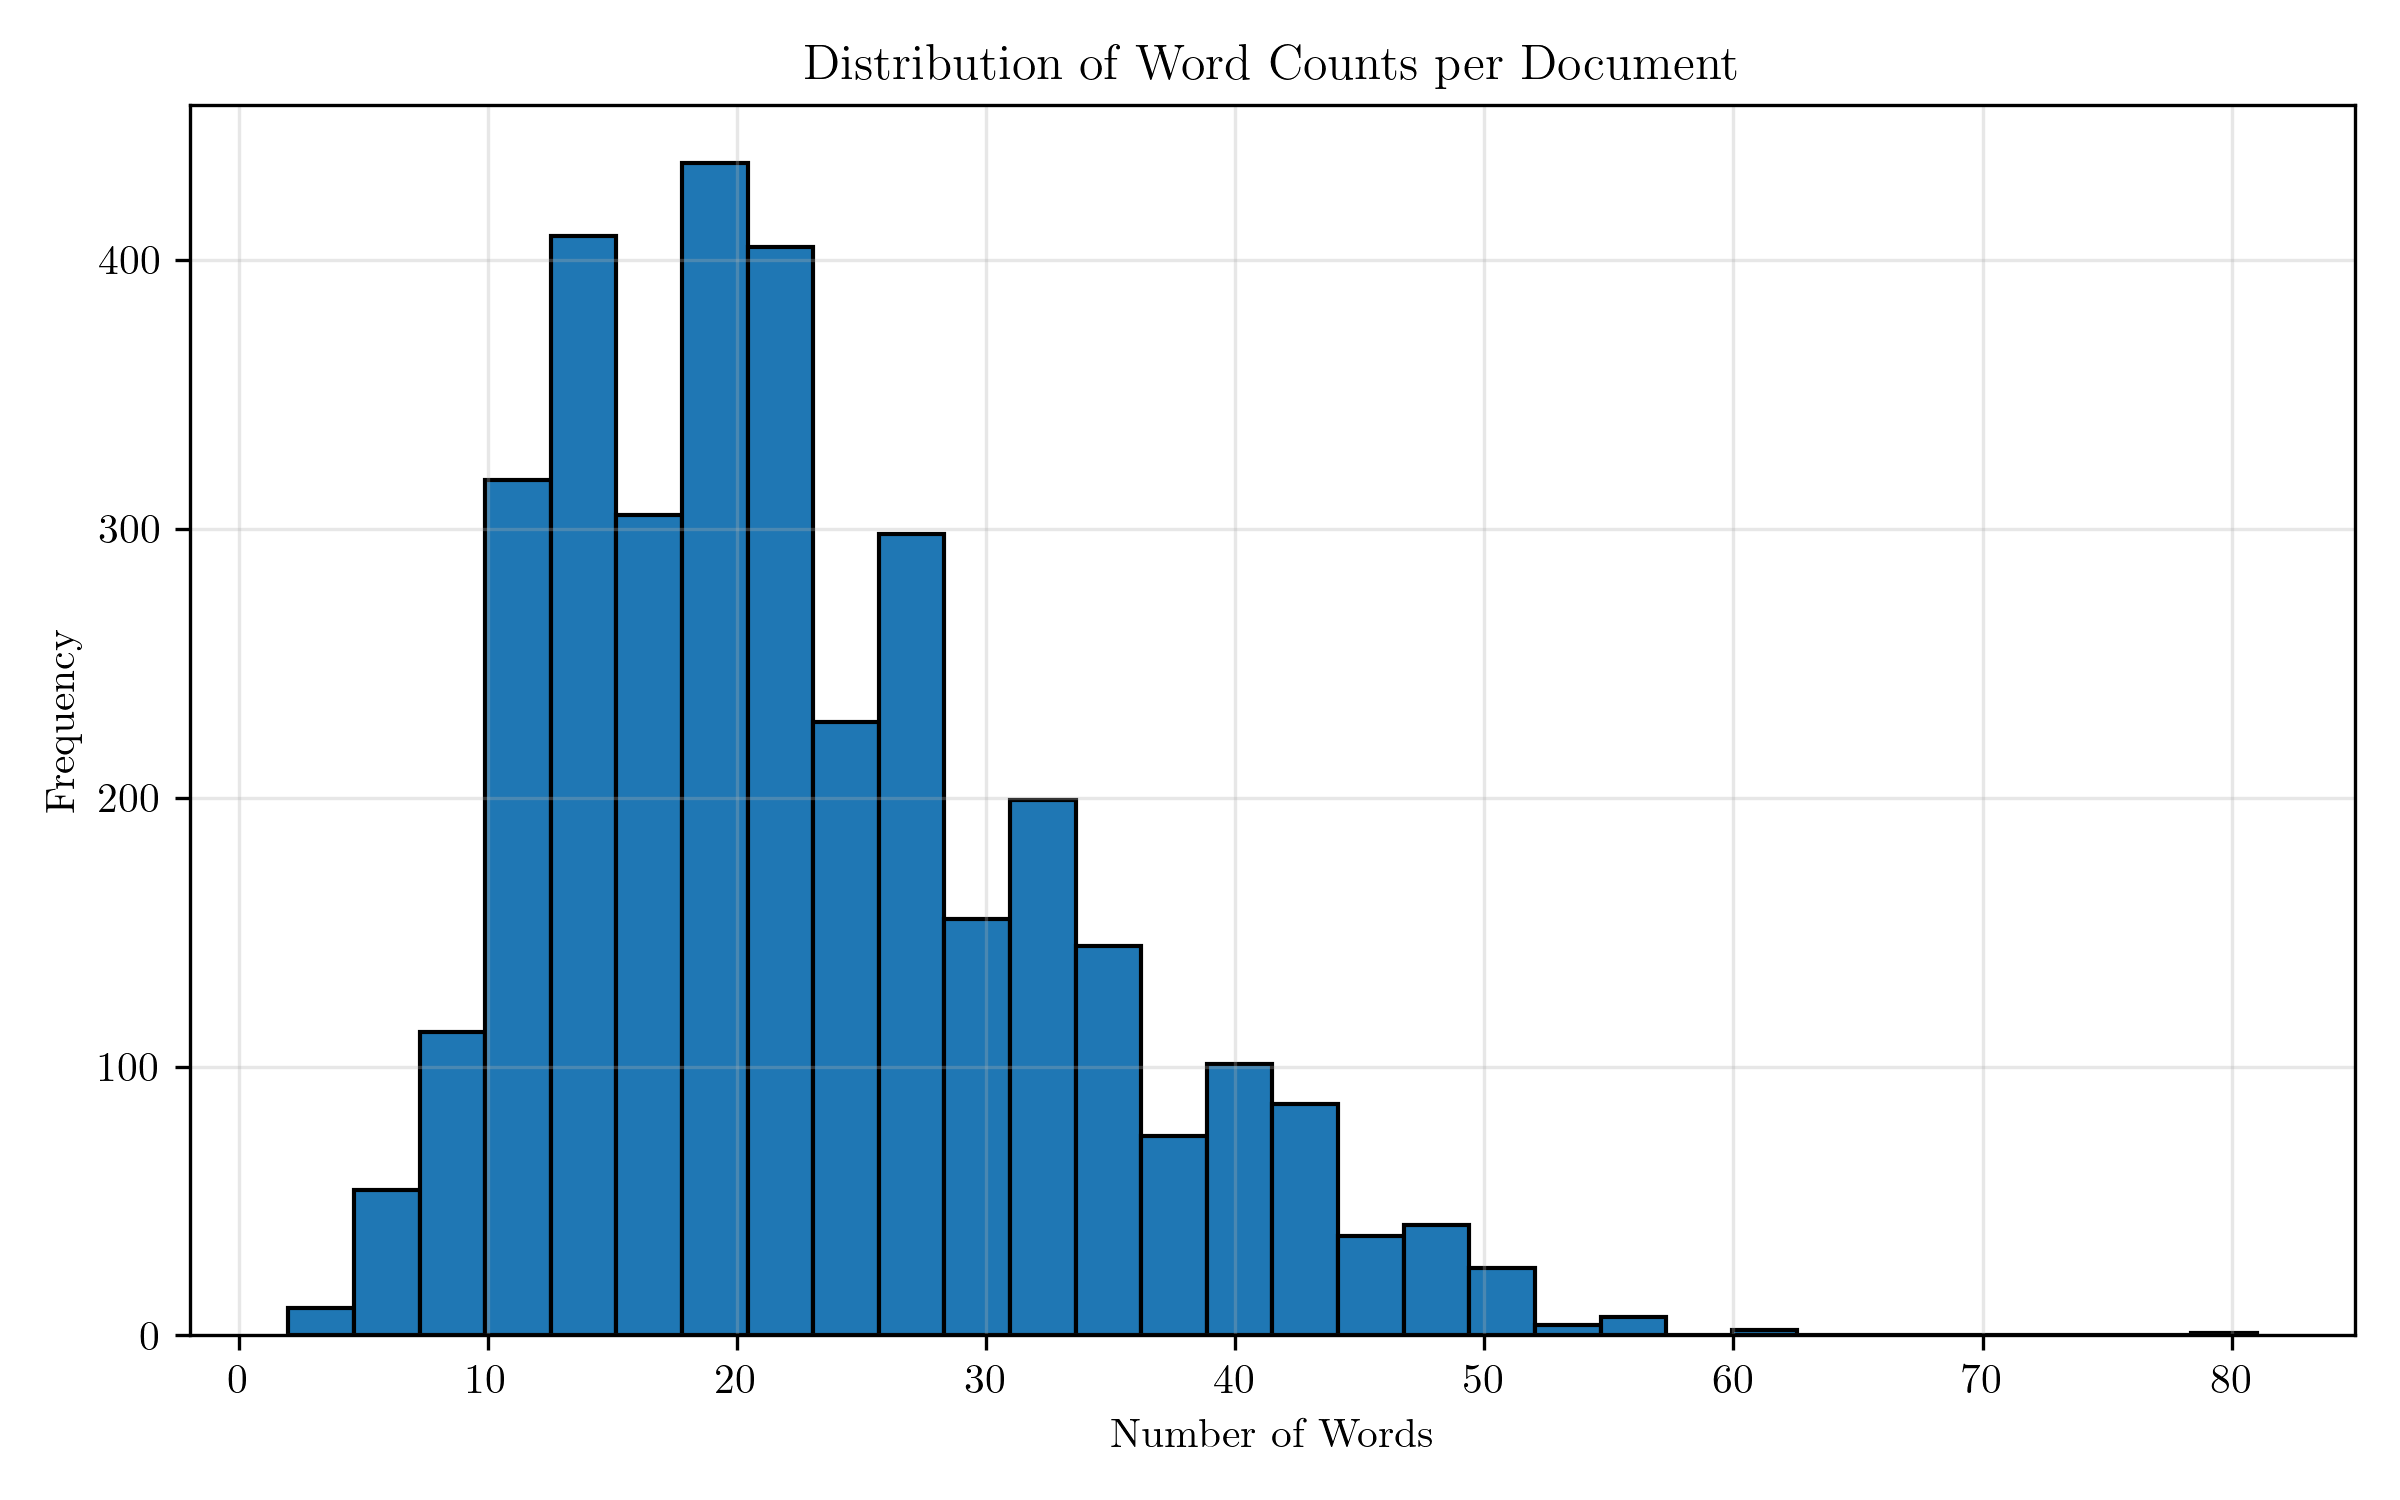
\includegraphics[width=1\linewidth]{assets/word_count_distribution.png}
    \caption{word count distribution}
    \label{fig:word_count_distribution}
\end{figure}

\begin{figure}[H]
    \centering
    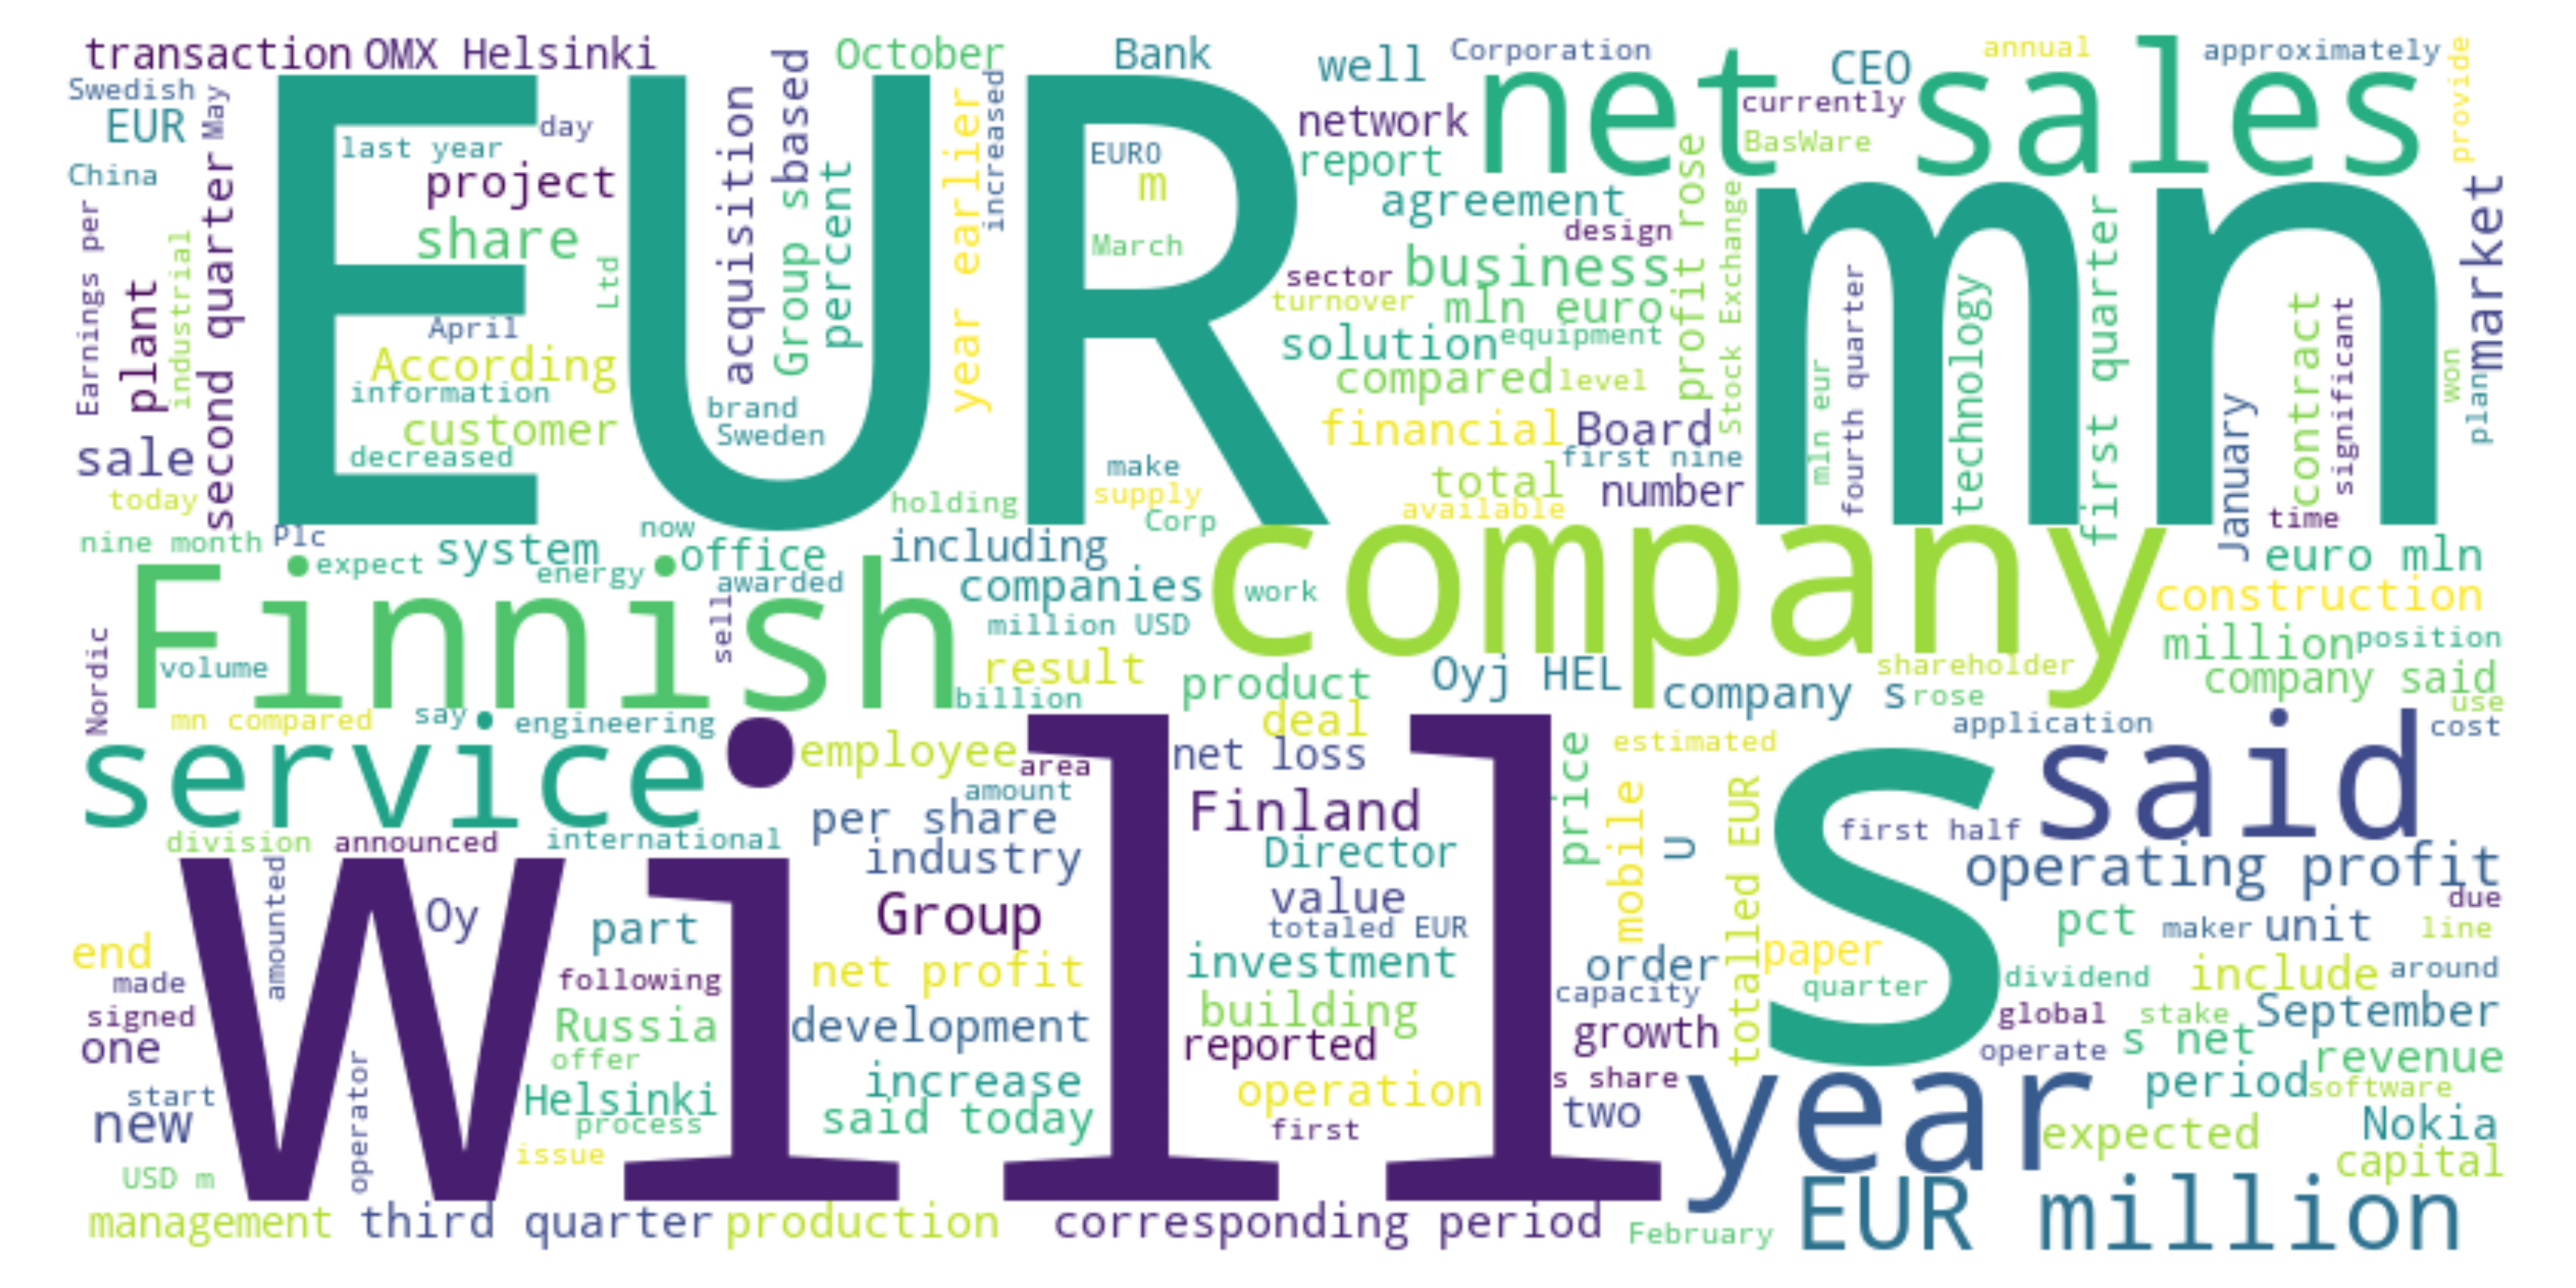
\includegraphics[width=1\linewidth]{assets/word_cloud_75agree.png}
    \caption{most common words in the sentences}
    \label{fig:word_cloud_75agree}
\end{figure}

most relevant words for class identification by checking which words appear much more in one class than others: down, decreased, profit, fell, rose


\subsection{Preprocessing}

split teste e treino

\section{Models}

abcbdhdhhd

\subsection{model 1}

model 1


\subsection{model 2}

model 2

\subsection{model 3}

model 3

\section{Exploring BERT}

\subsection{base model}

\begin{table}[H]
\centering
\caption{Hyperparameter space for ......}
\label{parameters_basebert}
\begin{tabular}{ll}
\toprule
\textbf{Hyperparameter} & \textbf{Possible Values} \\
\midrule
Epochs & $\{1,2,3,4,5\}$ \\
Learning rate & $[10^{-5}, 10^{-2}]$ \\
Weight decay & $[0, 0.5]$ \\
\bottomrule
\end{tabular}
\end{table}

best hyperameters: 

- Num train epochs: 2

- Learning rate: 0.0001

- Weight decay: 0.1

\begin{figure}[H]
    \centering
    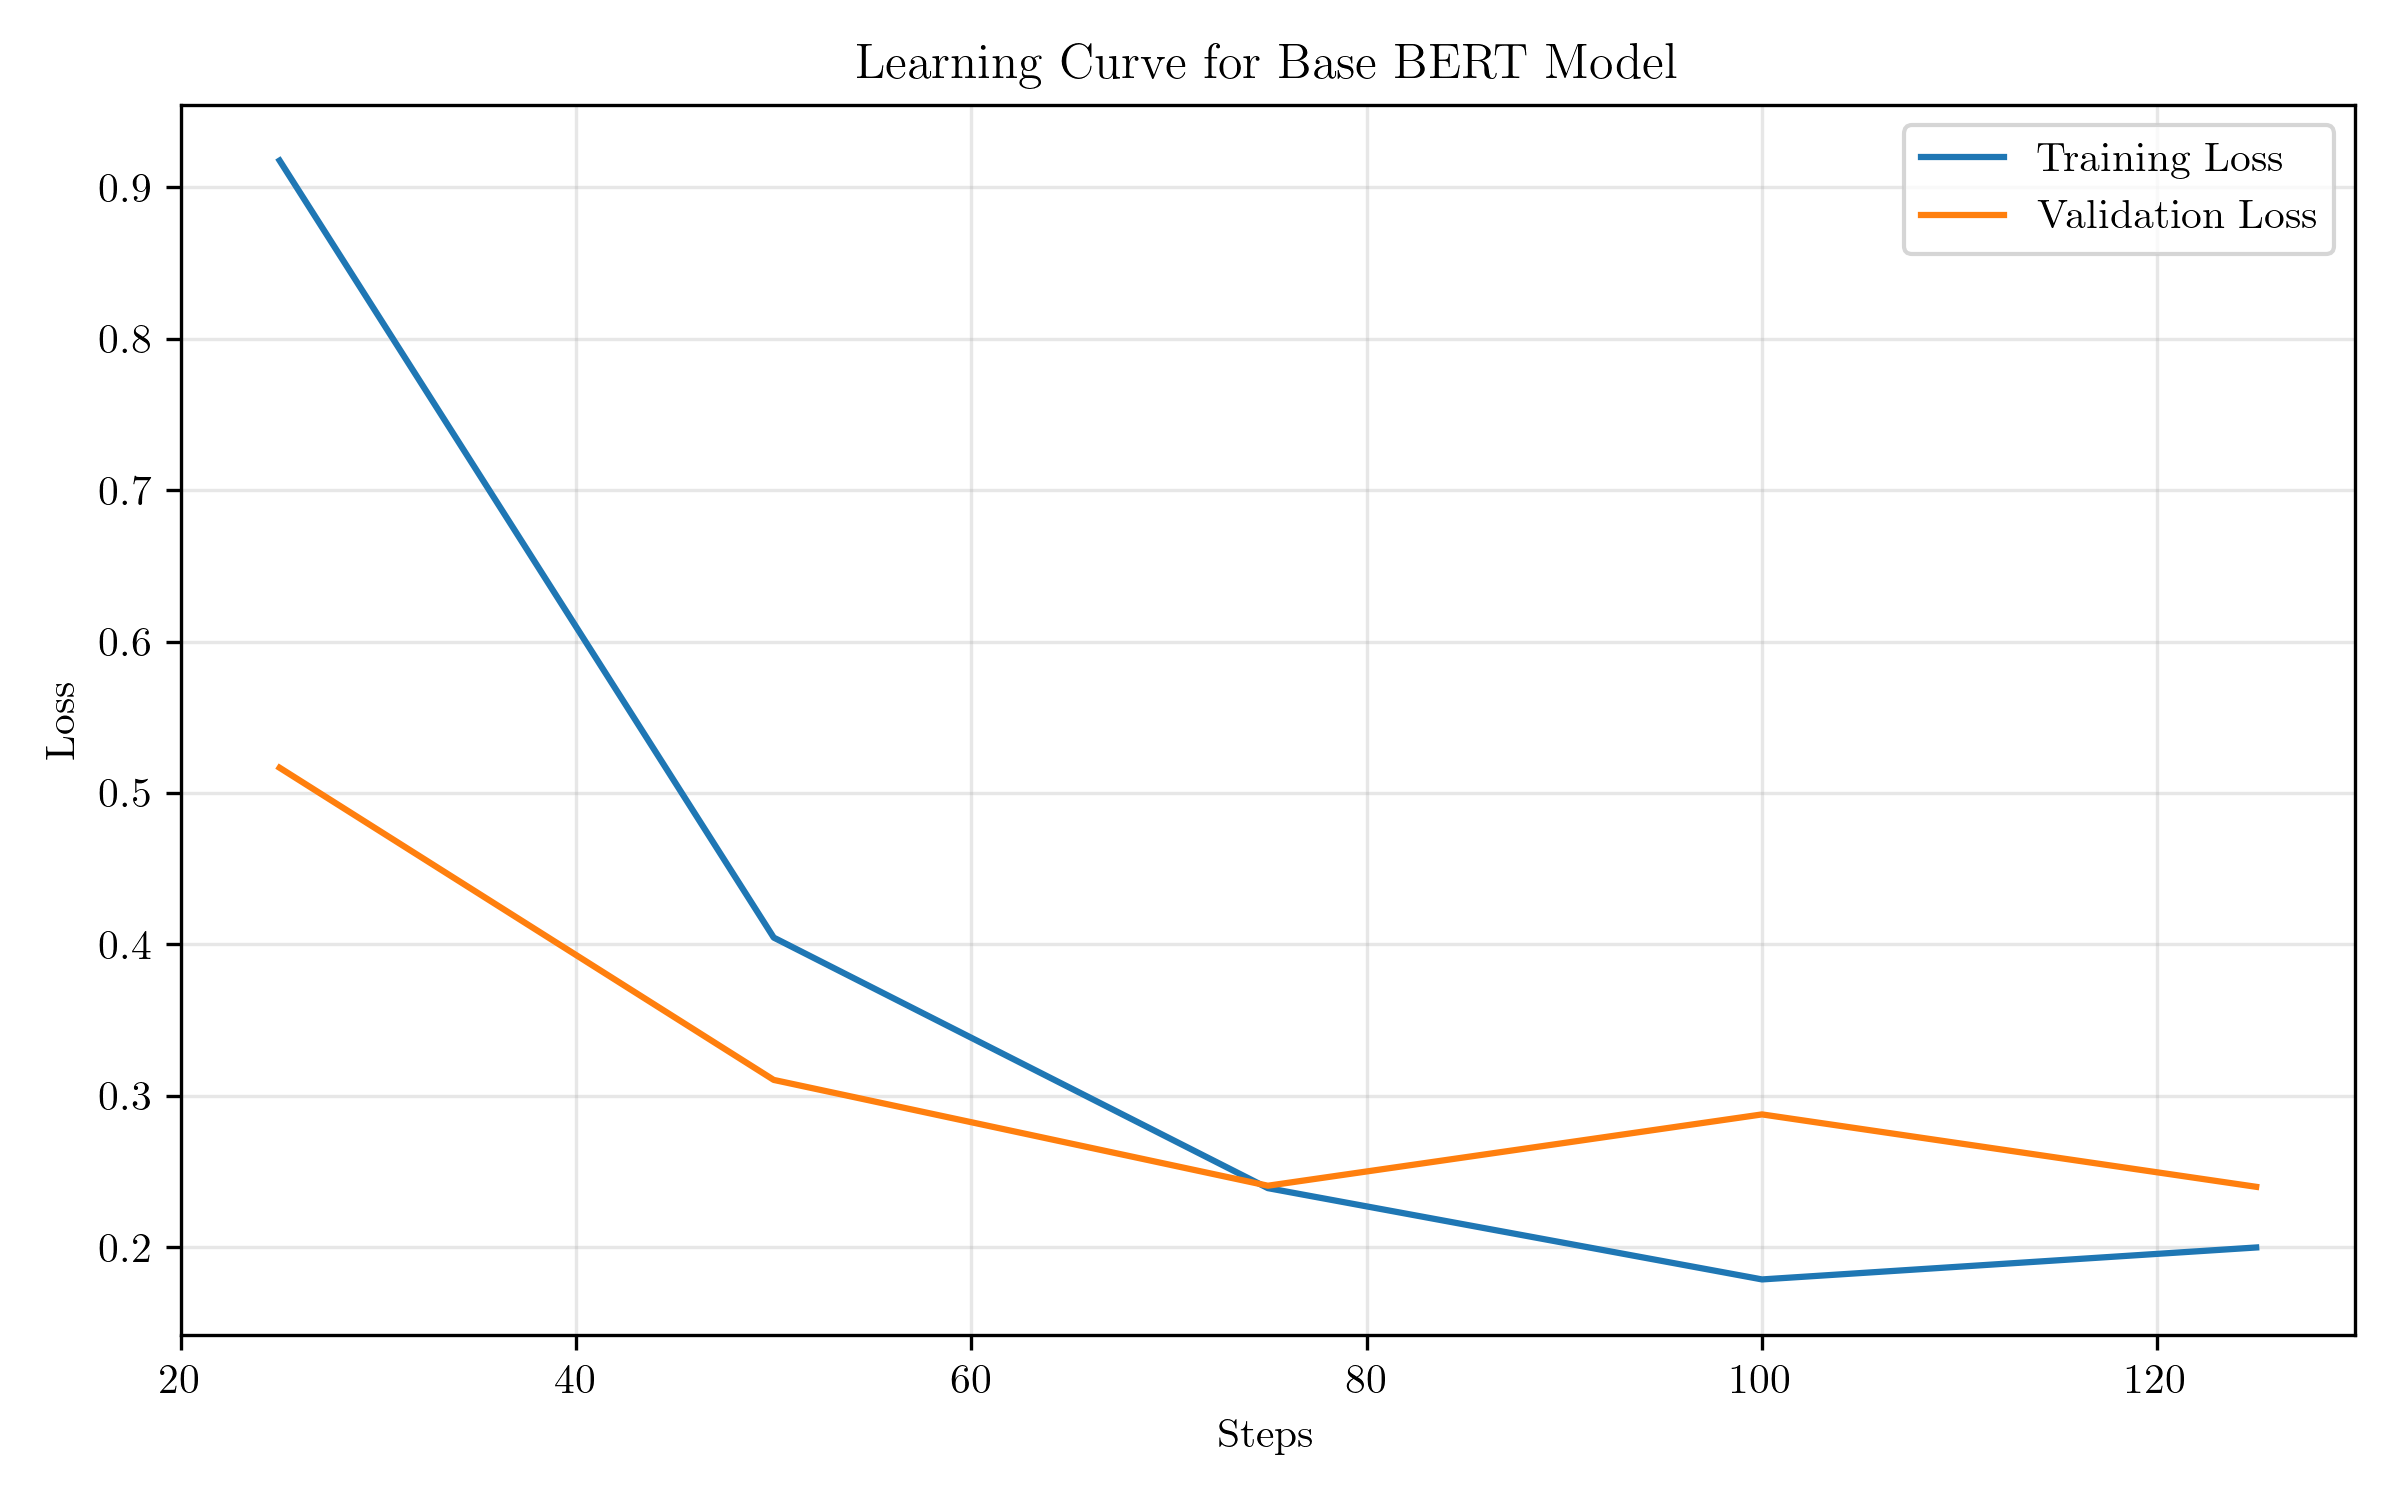
\includegraphics[width=1\linewidth]{assets/base_bert_learning_curve.png}
    \caption{learning curve}
    \label{fig:base_bert_learning_curve}
\end{figure}

\begin{figure}[H]
    \centering
    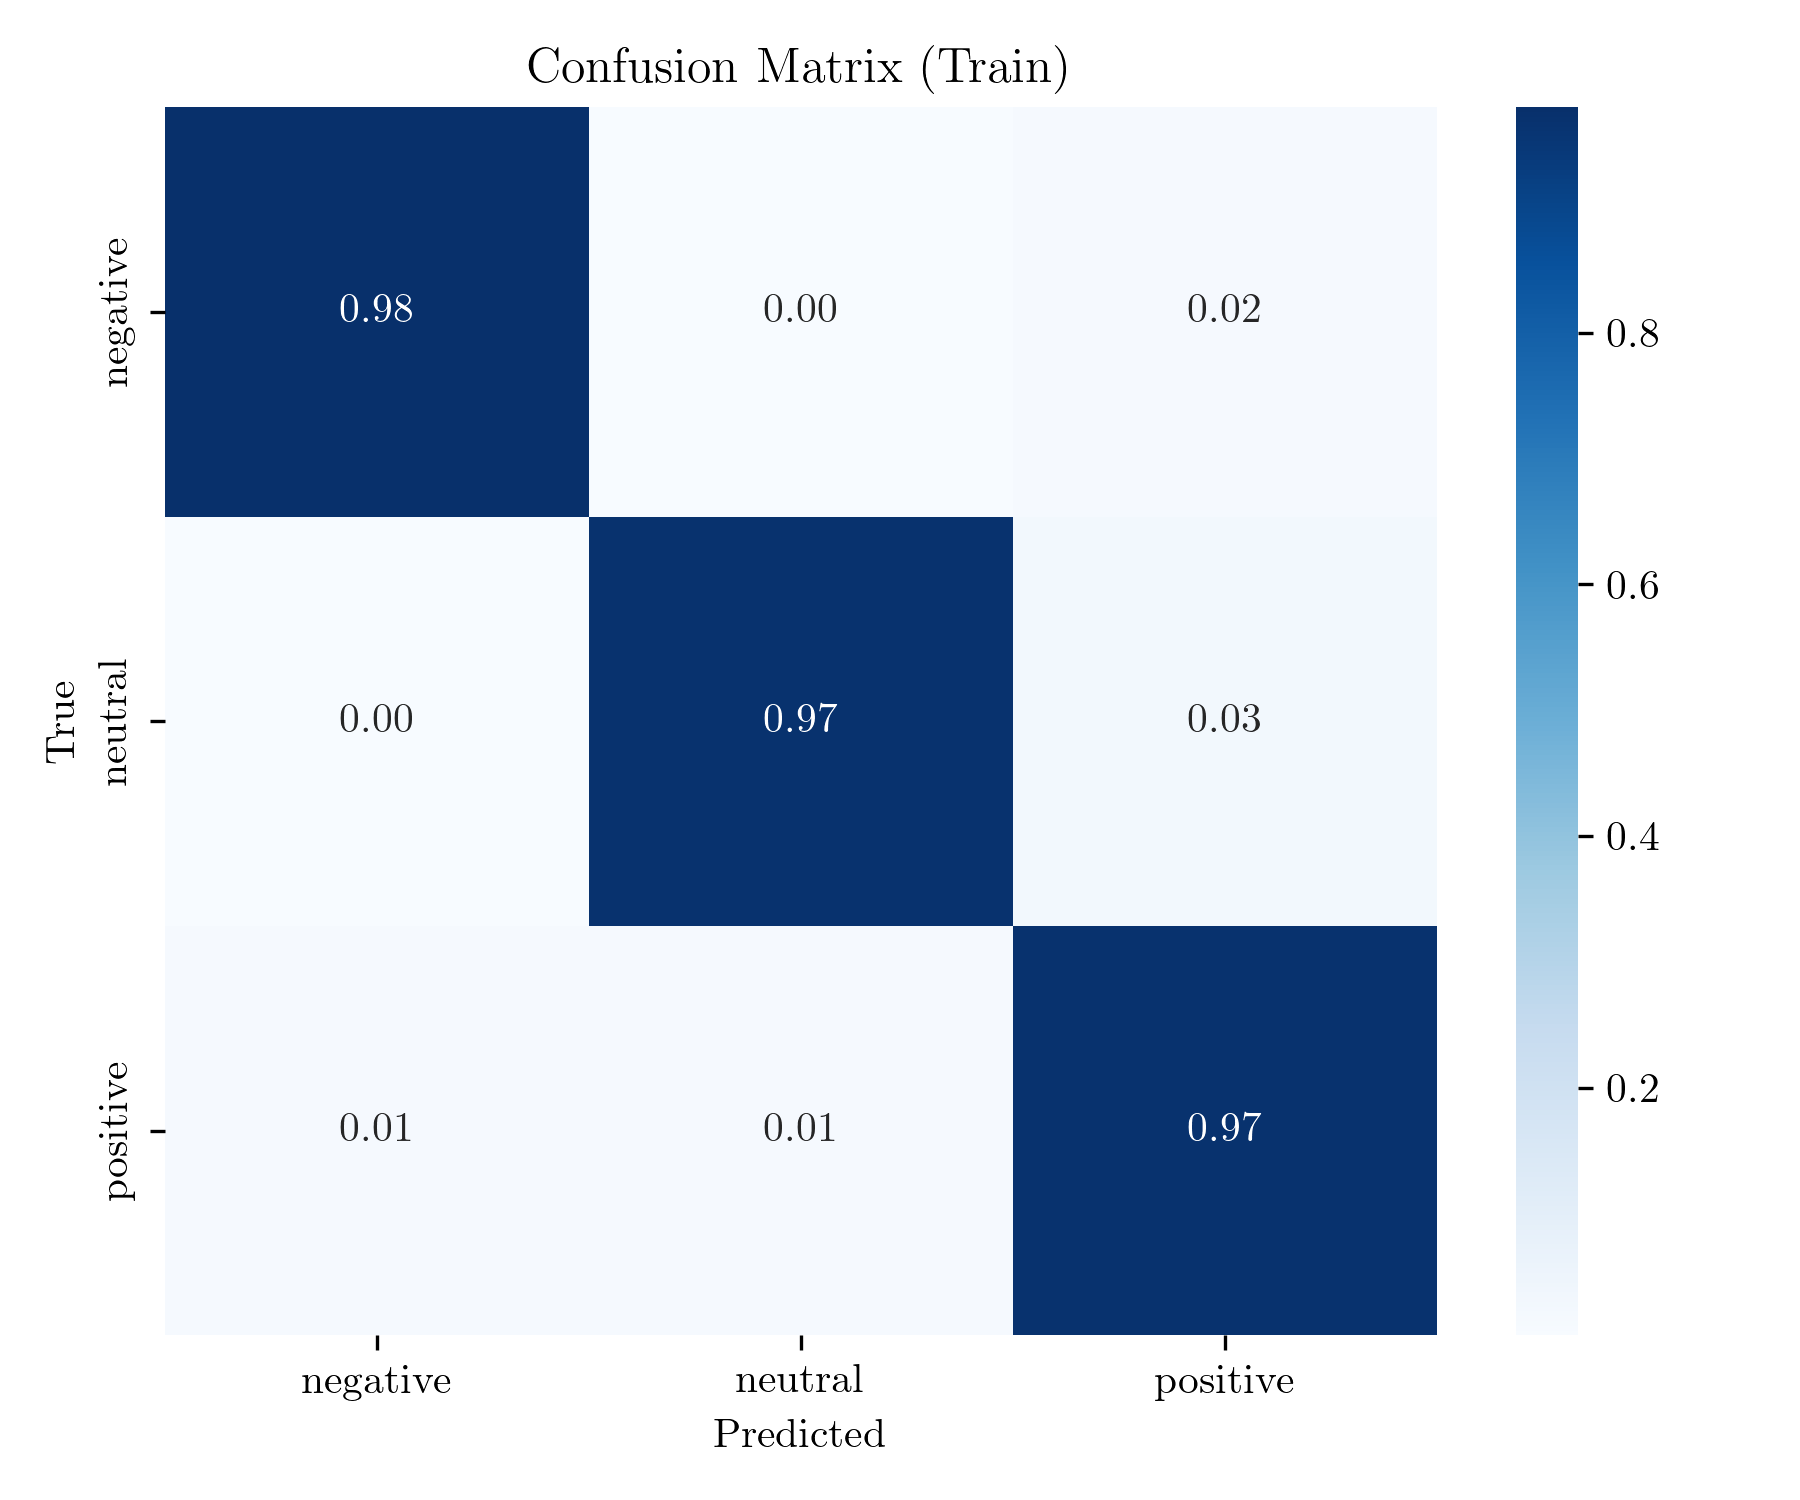
\includegraphics[width=1\linewidth]{assets/base_bert_confusion_matrix_Train.png}
    \caption{base bert conf matri train}
    \label{fig:base_bert_confusion_matrix_Train}
\end{figure}

\begin{table}[H]
\centering
\caption{Classification report for BASE BERT on training data.}
\label{cr_basebert_train}
\begin{tabular}{lcccccc}
\toprule
\textbf{Class} & \textbf{Precision} & \textbf{Recall} & \textbf{F1-Score} & \textbf{Support} \\
\midrule
Negative & 0.98 & 0.98 & 0.98 & 336 \\
Neutral & 0.98 & 0.97 & 0.98 & 336 \\
Positive & 0.96 & 0.97 & 0.96 & 336 \\
\midrule
\textbf{Accuracy} &  &  & 0.97 & 1008 \\
\textbf{Macro avg} & 0.97 & 0.97 & 0.97 & 1008 \\
\textbf{Weighted avg} & 0.97 & 0.97 & 0.97 & 1008 \\
\bottomrule
\end{tabular}
\end{table}

\begin{figure}[H]
    \centering
    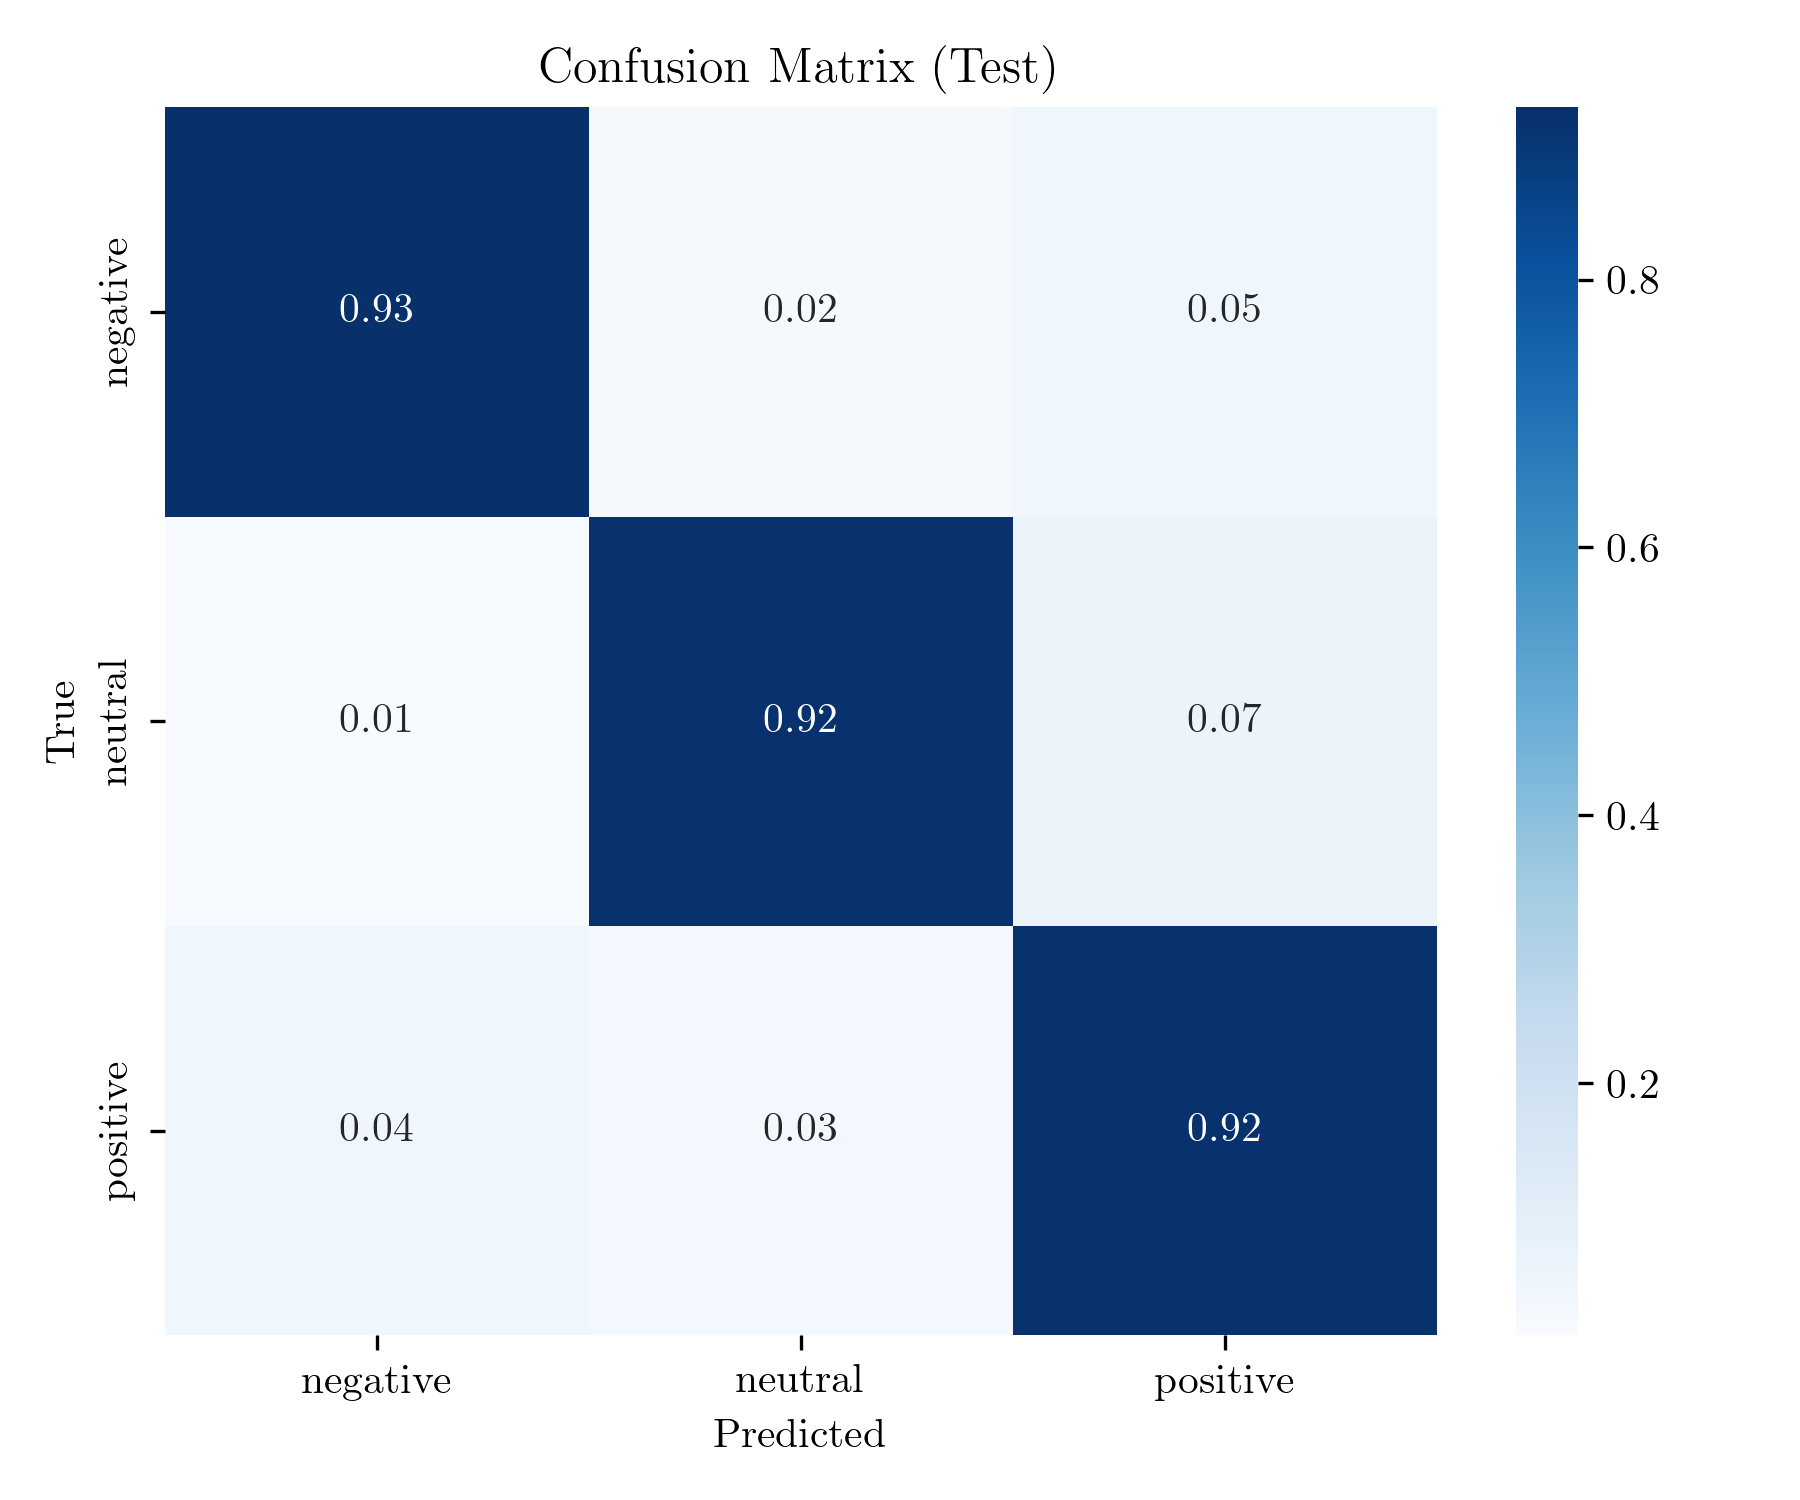
\includegraphics[width=1\linewidth]{assets/base_bert_confusion_matrix_Test.png}
    \caption{base bert cong matrix test}
    \label{fig:base_bert_confusion_matrix_Test}
\end{figure}

\begin{table}[H]
\centering
\caption{Classification report for BASE BERT on test data.}
\label{cr_basebert_test}
\begin{tabular}{lcccccc}
\toprule
\textbf{Class} & \textbf{Precision} & \textbf{Recall} & \textbf{F1-Score} & \textbf{Support} \\
\midrule
Negative & 0.86 & 0.93 & 0.89 & 84 \\
Neutral & 0.98 & 0.92 & 0.95 & 429 \\
Positive & 0.84 & 0.92 & 0.88 & 178 \\
\midrule
\textbf{Accuracy} &  &  & 0.92 & 691 \\
\textbf{Macro avg} & 0.89 & 0.92 & 0.91 & 691 \\
\textbf{Weighted avg} & 0.93 & 0.92 & 0.92 & 691 \\
\bottomrule
\end{tabular}
\end{table}


\section{Discussion}

results discuttion

eemplo de comparacao

\begin{table}[H]
\centering
\caption{Error metric (MAE) for the fine-tuned models, along with the best performers in the competition.}
\label{tab:model02_results_transposed}
\begin{tabular}{lr}
\toprule
\textbf{Model} & \textbf{MAE (Test Set)} \\
\midrule
Hybrid & 0.8434 \\
Obj. Det. & 1.2645 \\
Inst. Seg. & 1.3415 \\
Team Lacuna (1st) & 0.3299 \\
K\_Junior (2nd) & 0.5698 \\
\bottomrule
\end{tabular}
\end{table}




\section{Conclusion}

conclisao

\begin{figure}[H]
    \centering
    
\includegraphics[width=0.5\linewidth]{image.png}
    \caption{Enter Caption}
    \label{fig:enter-label}
\end{figure}
\section*{Work Load}

Both authors contributed equally to the project.

\bibliographystyle{IEEEtran}
\bibliography{references}

\end{document}



